%!Mode:: "TeX:UTF-8"
\documentclass[a4paper,11pt,UTF8]{ctexart}

\usepackage{indentfirst} %缩进
\usepackage{xeCJK}    %使用系统字体
\usepackage{fancyhdr} %自定义页眉页脚
\pagestyle{empty}                   %不设置页眉页脚
\usepackage{amsmath, amsthm, amssymb, amsfonts} %数学公式
\usepackage[a4paper,left=3cm,right=3cm,top=3cm,bottom=3cm]{geometry}
%\usepackage[tmargin=1in,bmargin=1in,lmargin=1.25in,rmargin=1.25in]{geometry}.
\usepackage{booktabs} %插入表格
\usepackage[section]{placeins} %避免浮动
\usepackage{listings} %插入代码
\usepackage{ctex}     %中文宏包
\usepackage[svgnames, table]{xcolor} %彩色表格
\usepackage{algorithm}          %伪代码
\usepackage{algorithmicx}
\usepackage{algpseudocode}
\usepackage{algorithm,algpseudocode,float}
\usepackage{lipsum}
\usepackage{enumitem}           %调整列举环境
\usepackage{url}
\usepackage{fontspec,xunicode}
\usepackage{float}
\defaultfontfeatures{Mapping=tex-text} %如果没有它,会有一些 tex 特殊字符无法正常使用,比如连字符。

\usepackage{graphicx}
\graphicspath{{imgs/}}

%%%%%%%%%%%%%%%%%%%%%%%%%%%%%%%%%%%%%%%%%%%%%%%%%%%%%%%%%%%%%%%%
% 缩进及行间距
%%%%%%%%%%%%%%%%%%%%%%%%%%%%%%%%%%%%%%%%%%%%%%%%%%%%%%%%%%%%%%%%
\setlength{\parindent}{22pt} %重新定义缩进长度
\setlength{\baselineskip}{20pt}  %定义行间距
%\renewcommand{\baselinestretch}{1.1} %定义行间距

%%%%%%%%%%%%%%%%%%%%%%%%%%%%%%%%%%%%%%%%%%%%%%%%%%%%%%%%%%%%%%%%
% 列表设置
%%%%%%%%%%%%%%%%%%%%%%%%%%%%%%%%%%%%%%%%%%%%%%%%%%%%%%%%%%%%%%%%
\setenumerate{fullwidth,itemindent=\parindent,listparindent=\parindent,itemsep=0ex,partopsep=0pt,parsep=0ex}
\setenumerate[2]{label=\alph*),leftmargin=1.5em}  %二级item设置
\setitemize{itemindent=38pt,leftmargin=0pt,itemsep=-0.4ex,listparindent=26pt,partopsep=0pt,parsep=0.5ex,topsep=-0.25ex}
\setdescription{itemindent=38pt,leftmargin=0pt,itemsep=-0.4ex,listparindent=26pt,partopsep=0pt,parsep=0.5ex,topsep=-0.25ex}

%%%%%%%%%%%%%%%%%%%%%%%%%%%%%%%%%%%%%%%%%%%%%%%%%%%%%%%%%%%%%%%%
% 图的标题行间距设置
%%%%%%%%%%%%%%%%%%%%%%%%%%%%%%%%%%%%%%%%%%%%%%%%%%%%%%%%%%%%%%%%
\newcommand{\bottomcaption}{%
\setlength{\abovecaptionskip}{6pt}%
\setlength{\belowcaptionskip}{6pt}%
\caption}


%%%%%%%%%%%%%%%%%%%%%%%%%%%%%%%%%%%%%%%%%%%%%%%%%%%%%%%%%%%%%%%%
% 字体定义
%%%%%%%%%%%%%%%%%%%%%%%%%%%%%%%%%%%%%%%%%%%%%%%%%%%%%%%%%%%%%%%%
\setmainfont{Times New Roman}  %默认英文字体.serif是有衬线字体sans serif无衬线字体
\setmonofont{Consolas}
\setCJKmainfont[ItalicFont={楷体}, BoldFont={黑体}]{宋体}%衬线字体 缺省中文字体为
\setCJKsansfont{黑体}
\punctstyle{hangmobanjiao}
%-----------------------xeCJK下设置中文字体------------------------------%
\setCJKfamilyfont{song}{SimSun}                             %宋体 song
\newcommand{\song}{\CJKfamily{song}}
\setCJKfamilyfont{fs}{FangSong}                      %仿宋  fs
\newcommand{\fs}{\CJKfamily{fs}}
\setCJKfamilyfont{ktgb}{KaiTi}                      %楷体2312 ktgb
\newcommand{\ktgb}{\CJKfamily{ktgb}}
\setCJKfamilyfont{yh}{Microsoft YaHei}                    %微软雅黑 yh
\newcommand{\yh}{\CJKfamily{yh}}
\setCJKfamilyfont{hei}{SimHei}                              %黑体  hei
\newcommand{\hei}{\CJKfamily{hei}}
\setCJKfamilyfont{hwxk}{STXingkai}                                %华文行楷  hwxk
\newcommand{\hwxk}{\CJKfamily{hwxk}}
%------------------------------设置字体大小------------------------%
\newcommand{\shiyanbaogao}{\fontsize{36pt}{\baselineskip}\selectfont}
\newcommand{\chuhao}{\fontsize{42pt}{\baselineskip}\selectfont}     %初号
\newcommand{\xiaochuhao}{\fontsize{36pt}{\baselineskip}\selectfont} %小初号
\newcommand{\yihao}{\fontsize{28pt}{\baselineskip}\selectfont}      %一号
\newcommand{\erhao}{\fontsize{21pt}{\baselineskip}\selectfont}      %二号
\newcommand{\xiaoerhao}{\fontsize{18pt}{\baselineskip}\selectfont}  %小二号
\newcommand{\sanhao}{\fontsize{15.75pt}{\baselineskip}\selectfont}  %三号
\newcommand{\sihao}{\fontsize{14pt}{\baselineskip}\selectfont}       %四号
\newcommand{\xiaosihao}{\fontsize{12pt}{\baselineskip}\selectfont}  %小四号
\newcommand{\wuhao}{\fontsize{10.5pt}{\baselineskip}\selectfont}    %五号
\newcommand{\xiaowuhao}{\fontsize{9pt}{\baselineskip}\selectfont}   %小五号
\newcommand{\liuhao}{\fontsize{7.875pt}{\baselineskip}\selectfont}  %六号
\newcommand{\qihao}{\fontsize{5.25pt}{\baselineskip}\selectfont}    %七号

%%%%%%%%%%%%%%%%%%%%%%%%%%%%%%%%%%%%%%%%%%%%%%%%%%%%%%%%%%%%%%%%
% 图题字体大小相同
%%%%%%%%%%%%%%%%%%%%%%%%%%%%%%%%%%%%%%%%%%%%%%%%%%%%%%%%%%%%%%%%
\usepackage{caption}
\captionsetup{font={footnotesize}}   % footnotesize = 9pt
\captionsetup[lstlisting]{font={footnotesize}}

%%%%%%%%%%%%%%%%%%%%%%%%%%%%%%%%%%%%%%%%%%%%%%%%%%%%%%%%%%%%%%%%
% 重定义枚举编号为 1),2)...
%%%%%%%%%%%%%%%%%%%%%%%%%%%%%%%%%%%%%%%%%%%%%%%%%%%%%%%%%%%%%%%%
\renewcommand{\labelenumi}{\theenumi)}


%%%%%%%%%%%%%%%%%%%%%%%%%%%%%%%%%%%%%%%%%%%%%%%%%%%%%%%%%%%%%%%%
% 重定义section标题
%%%%%%%%%%%%%%%%%%%%%%%%%%%%%%%%%%%%%%%%%%%%%%%%%%%%%%%%%%%%%%%%
\CTEXsetup[format={\sihao\CJKfamily{zhhei}\zihao{4}},number={\chinese{section}},name={,、~},aftername={},indent={0pt},beforeskip={6pt},afterskip={6pt},format+={\flushleft}]{section}
\CTEXsetup[format={\Large\bfseries\CJKfamily{zhkai}\zihao{5}},name={(,)},number={\chinese{subsection}},aftername={},indent={22pt},beforeskip={14pt},afterskip={2pt}]{subsection}
\CTEXsetup[number={\chinese{section}},name={附录, ~~ }]{appendix}



%%%%%%%%%%%%%%%%%%%%%%%%%%%%%%%%%%%%%%%%%%%%%%%%%%%%%%%%%%%%%%%%
% 标题名称中文化
%%%%%%%%%%%%%%%%%%%%%%%%%%%%%%%%%%%%%%%%%%%%%%%%%%%%%%%%%%%%%%%%
\renewcommand\figurename{\hei 图}
\renewcommand\tablename{\hei 表}
\renewcommand\lstlistingname{\hei 代码}
\renewcommand{\algorithmicrequire}{\textbf{输入:}}
\renewcommand{\algorithmicensure}{\textbf{输出:}}
\newtheorem{define}{定义}

%%%%%%%%%%%%%%%%%%%%%%%%%%%%%%%%%%%%%%%%%%%%%%%%%%%%%%%%%%%%%%%%
% 代码设置
%%%%%%%%%%%%%%%%%%%%%%%%%%%%%%%%%%%%%%%%%%%%%%%%%%%%%%%%%%%%%%%%
\lstset{
 columns=fixed,
 numbers=left,                                        % 在左侧显示行号
 numberstyle=\tiny\color{gray},                       % 设定行号格式
 frame=single,                                        % 单线背景边框
 breaklines=true,                                     % 设定LaTeX对过长的代码行进行自动换行
 keywordstyle=\color[RGB]{40,40,255},                 % 设定关键字颜色
 numberstyle=\footnotesize\color{darkgray},
 commentstyle=\it\color[RGB]{0,96,96},                % 设置代码注释的格式
 stringstyle=\rmfamily\slshape\color[RGB]{128,0,0},   % 设置字符串格式
 showstringspaces=false,                              % 不显示字符串中的空格
 language=java,                                        % 设置语言
 basicstyle=\linespread{1.0}\xiaowuhao\ttfamily,                      % 字体字号
 %lineskip=10pt,
 %baselinestretch=1,
}

%%%%%%%%%%%%%%%%%%%%%%%%%%%%%%%%%%%%%%%%%%%%%%%%%%%%%%%%%%%%%%%%
% 伪代码分页
%%%%%%%%%%%%%%%%%%%%%%%%%%%%%%%%%%%%%%%%%%%%%%%%%%%%%%%%%%%%%%%%
\makeatletter
\renewcommand{\ALG@name}{算法}
\newenvironment{breakablealgorithm}
  {% \begin{breakablealgorithm}
   \begin{center}
     \refstepcounter{algorithm}% New algorithm
     \hrule height.8pt depth0pt \kern2pt% \@fs@pre for \@fs@ruled
     \renewcommand{\caption}[2][\relax]{% Make a new \caption
       {\raggedright\textbf{\ALG@name~\thealgorithm} ##2\par}%
       \ifx\relax##1\relax % #1 is \relax
         \addcontentsline{loa}{algorithm}{\protect\numberline{\thealgorithm}##2}%
       \else % #1 is not \relax
         \addcontentsline{loa}{algorithm}{\protect\numberline{\thealgorithm}##1}%
       \fi
       \kern2pt\hrule\kern2pt
     }
  }{% \end{breakablealgorithm}
     \kern2pt\hrule\relax% \@fs@post for \@fs@ruled
   \end{center}
  }
\makeatother



\begin{document}
\xiaosihao\song

\begin{titlepage}
\center{\yihao{\hwxk{武汉大学国家网络安全学院}}}
\vspace{6cm}
\center{\shiyanbaogao{\ktgb{信~息~隐~藏~实~验~报~告}}}
\vspace{4cm}

\begin{center}
\begin{large}
\begin{tabular}{rc}
\xiaoerhao{\hei{学\qquad 号}}& \hspace{1.7cm}\xiaoerhao{\hei{2021302181156\hspace{1.7cm}}} \\
\cline{2-2}\\
\xiaoerhao{\hei{姓\qquad 名}}& \xiaoerhao{\hei{赵~伯~俣}}\\
\cline{2-2}\\
\xiaoerhao{\hei{实验名称}}& \xiaoerhao{\hei{安~全~隐~写~对~抗~技~术}}\\
\cline{2-2}\\
\xiaoerhao{\hei{指导教师}}& \xiaoerhao{\hei{任~延~珍}}\\
\cline{2-2}
\end{tabular}
\end{large}
\end{center}
\vfill \hfill
\end{titlepage}
\clearpage

% \centerline{\\[10pt]\erhao{\fs{武 ~汉 ~ 大~ 学}}}
% \centerline{\\[10pt]\yihao{\fs{信~息~隐~藏~实~验~报~告}}}

% \leftline{\\[10pt]\sihao{\hei{\hspace{1.5em} 学生姓名:XXX \hfill 学号:XXXX \hfill 指导教师:XXX }}}

% \leftline{\\[10pt]\sihao{\hei{\hspace{1.5em} 实验地点:新珈楼XXX \hfill }}}

% \leftline{\\[10pt]\sihao{\hei{\hspace{1.5em} 实验时间:第X周周X(X-X节) \hfill }}}



\setlength{\parskip}{6pt}  %定义段间距

\section{实验名称: 安~全~隐~写~对~抗~技~术}

\section{实验目的:}

  1.实现LSBM隐写算法的消息嵌入和提取并分析其安全性\\
  \hspace*{22pt}2.实现卡方分析,并且利用卡方分析检测不同嵌入率下LSBR和LSBM的情况,进行对比分析\\
  \hspace*{22pt}3.实现F4隐写算法的消息嵌入和提取并分析其安全性\\
  \hspace*{22pt}4.实现F5隐写算法的消息嵌入和提取并分析其安全性

\section{实验原理:}

  \subsection{LSBM隐写算法}
    为了克服在LSBR算法中产生的值对效应,当载体图像的LSB与消息比特不同时,将像素值随机加减1,
    且为了防止溢出,当载体像素值为0时,则进行加1操作,若像素值为255,则进行减1操作,对于其他的
    载体像素值则随机进行加1或者减1。从而避免偶数只能加1变成奇数和奇数只能减1变成偶数的值对效应。

  \subsection{卡方分析}
    针对图像像素LSB全嵌入的情况,利用数理统计假设检验中的卡方检验模型来分析统计样本的实际观测值
    与理论推断值之间的偏离程度,决定卡方值的大小,如果卡方值越大,二者的偏差程度越大,反之,
    二者偏差越小;若两者完全相等时,卡方值就为0,表明理论值完全符合\par
    设图像中灰度值为i的像素数量为h{\scriptsize i},其中i的取值为 $[0,127]$\par
    对于任意一组奇偶灰度值2i和2i+1,其对应的像素块数目为h{\scriptsize 2i}和h{\scriptsize 2i+1},
    将任意一组奇偶灰度值的平均值设置为y{\scriptsize 1},将二者的差定义为y{\scriptsize 2}
    通过比较y{\scriptsize 1}和y{\scriptsize 2}之间的偏离程度来计算卡方统计量,\par
    由此可得定义变量t=$\sum_{i=1}^{127} \frac{\left ( h{2i-1} -h{2i} \right )^{2} }{2\times \left (h{2i-1}+h{2i}\right ) }$\\
    t满足自由度为 v=d-1的卡方分布,
    由此可以计算得到自由度为V的卡方分布在x点处的分布函数值即$F\left ( x<X \right ) $\par
    为了使结果更加明显定义变量p代表当前图像被隐写概率$p=1-F\left ( x<X \right ) $\par
    同时为了能够分析出图像的嵌入率,在计算卡方分析时需要将图像按行分成10份,每10\%计算一次p,
    通过观察p在何时值变小来确定图像的嵌入率

  \subsection{F4隐写算法}
    用秘密信息比特替换JPEG图像量化后的DCT系数的LSB,但不处理为0的DCT系数,从而保证在隐写后人眼无法分辨隐写图
    和原图的差别。\par
    为了避免在jsteg隐写过程中出现的值对效应和在F3隐写中出现的偶系数增多的缺点,在F4中使用全新的替换策略:
    在提取时只需要将AC系数中的非0位正奇数和负偶数代表1,正偶数和负奇数代表0。

  \subsection{F5隐写算法}
    F5隐写算法用秘密信息比特替换JPEG图像量化后的DCT系数的LSB,但不处理为0的DCT系数,从而保证在隐写后人眼无法分辨隐写图
    和原图的差别。\par
    另外F5隐写算法使用了矩阵编码即汉明码的方法,在嵌入过程中使用到了汉明码的一致校验阵,嵌入规则采用与F4相同的嵌入规则。
    矩阵编码的目的就是通过编码的方式减少每个载体分组中所需要的嵌入修改次数,提高嵌入效率,
    使每个LSB修改可以嵌入更多的秘密比特。\par
    在嵌入时首先选取7位载体矩阵a,将其与汉明码的一致校验阵进行矩阵乘法运算得到c,将c按位模2后将其视为8进制转换为10进制,
    得到将要修改的位r,若r=0则不需要对载体矩阵a进行修改,若r不为0则修改载体矩阵a中的第r位得到修改后的载体矩阵。\par
    在提取时将修改后的载体矩阵与汉明码一致校验阵进行矩阵乘法运算后即可得到隐藏的信息。\par
    在进行位置置乱时采用Arnold变换对隐写前的图像进行在有限区域内进行反复折叠、拉伸变换,该变换采用的算法如下所示 \par
    $\begin{bmatrix}y{n+1 }  \\x{ n+1}  \end{bmatrix}=\begin{bmatrix}1  &b \\a  &ab+1\end{bmatrix}\begin{bmatrix}y{n}  \\x{ n} \end{bmatrix}$\par
    在隐写结束后以及DCT逆变换之前,需要将图像的位置置乱进行还原,位置置乱的还原算法如下所示\par
    $\begin{bmatrix}y{ n+1 }  \\x{n+1}  \end{bmatrix}=\begin{bmatrix}ab+1  &-b \\-a  &1\end{bmatrix}\begin{bmatrix}y{n}  \\x{n} \end{bmatrix}$\par


\section{实验内容:}

  \subsection{实验1.1:LSBM隐写算法}
    LSBM信息隐藏的代码如代码1所示
    \lstinputlisting[caption={LSBM隐写代码},captionpos=b]{E:/matlab_codes/lab_2/LSBM/LSBM_hide.m} 
    LSBM信息提取的代码如代码2所示
    \lstinputlisting[caption={LSBM提取代码},captionpos=b]{E:/matlab_codes/lab_2/LSBM/LSBM_get.m} 
\newpage
    LSBM隐写过程中使用的随机加减的函数代码如代码3所示
    \lstinputlisting[caption={LSBM隐写随机加减代码},captionpos=b]{E:/matlab_codes/lab_2/LSBM/plus_or_sub.m} 
    
  \subsection{实验1.2:卡方分析}
    卡方分析代码如代码4所示
    \lstinputlisting[caption={k2分析代码},captionpos=b]{E:/matlab_codes/lab_2/k2/k2_disp.m} 
    在卡方分析中用到的LSBR隐写的算法如代码5所示
    \lstinputlisting[caption={LSBR隐写代码},captionpos=b]{E:/matlab_codes/lab_2/LSBR/LSBR_hide.m} 
    在卡方分析中用到的LSBR提取的算法如代码6所示
    \lstinputlisting[caption={LSBR提取代码},captionpos=b]{E:/matlab_codes/lab_2/LSBR/LSBR_get.m}

  \subsection{实验2.1:F4隐写算法}
    F4隐写算法的代码如代码7所示
    \lstinputlisting[caption={F4隐写代码},captionpos=b]{E:/matlab_codes/lab_2/F4/F4_hide.m}
    F4隐写信息提取的代码如代码8所示
    \lstinputlisting[caption={F4提取代码},captionpos=b]{E:/matlab_codes/lab_2/F4/F4_get.m}
\newpage
  \subsection{实验2.2:F5隐写算法}
    F5隐写算法的代码如代码9所示
    \lstinputlisting[caption={F5隐写代码},captionpos=b]{E:/matlab_codes/lab_2/F5/F5_hide.m}
    F5隐写信息提取的代码如代码10所示
    \lstinputlisting[caption={F5隐写信息提取代码},captionpos=b]{E:/matlab_codes/lab_2/F5/F5_get.m}

\section{实验环境:}

  1.win11操作系统\par
  2.MATLAB R2022a

\newpage
\section{实验步骤:}
    \subsection{实验1.1:LSBM隐写算法}
      \subsubsection{生成随机秘密消息}
        通过给出的嵌入率生成占到整个图像k倍的随机秘密信息矩阵,该矩阵通过调用函数ransrc生成。
      \subsubsection{在LSB位嵌入图像}
        遍历载体矩阵LSB位上的信息,如果与隐藏信息对应位的信息相同则不进行操作,如果与隐藏信息不同则
        判断载体上的像素值是否为0或225,如果是0则将其+1,如果是255则将其减1。如果像素值不为0或255
        则调用随机加减函数将该像素值进行随机加减1的操作。
      \subsubsection{绘制灰度图像直方图}
        调用函数imhist处理原灰度图和经过隐写后的灰度图像,对比隐写前后图像的值对效应。
      \subsubsection{隐藏信息的提取}
        在隐藏信息提取时,只需要注意在隐写后的图像的像素值若为奇数则提取1,若为偶数则提取2。

    \subsection{实验1.2:卡方分析}
      \subsubsection{载体图像分块}
        在进行卡方分析前,首先要对载体图像进行分块,在本次实验中将图像分成了10个小块,在之后的实验步骤中
        对每一块循环遍历计算相应的被隐写的概率
      \subsubsection{计算卡方统计量}
        在每一个小块中统计载体的灰度值为i的像素块的数量记录为h$\left ( i \right )$ ,其中i的取值范围为
        $ 0\le i\le 127$。\par
        由此可得统计量$x_i =\frac{\left ( h{2i-1}-h{2i}   \right ) ^{2} }{2\times \left ( h{2i-1} +h{2i}  \right ) } $
        服从自由度为1的卡方分布。\par
        将所有的$x_i$累加得到卡方统计值\par
      \subsubsection{计算被隐写概率}
        调用函数chi2cdf(X,V)计算自由度为V的卡方分布在X点处的分布函数值即$F\left ( x<X \right ) $\par
        最后统计p=1-$F\left ( x<X \right ) $的值作为当前小块的被隐写概率
      \subsubsection{绘制每一个小块的被隐写概率图像}
        最后将每一次循环遍历得到的小块的被隐写概率绘制成图像的形式观察该折线图的拐点即为图像的嵌入率

    \subsection{实验2.1:F4隐写算法}
      \subsubsection{载体图像分块做二维DCT变换}
        首先与DCT隐写相同,先规定量化矩阵的值,然后将图像划分成8*8的块,对每一块先调用dct2函数
        进行DCT变换,然后将其与量化矩阵做矩阵除法,将得到的结果取整数,得到的即为经过处理的DCT系数,
      \subsubsection{获取分块中的AC系数并进行信息隐写}
        将上一个步骤中得到的经过处理的DCT系数取出LSB位,即去掉每一块中最左上角的块,
        剩余的系数即为AC系数,在AC系数中进行信息隐写
        为了解决隐写过程中产生的值对效应和载密图像中偶系数增多的问题,在修改AC系数时采用如下规则进行信息的嵌入
        1.跳过0
        2.若AC系数为2i,且$i\ge 0$,秘密信息比特为0,则该AC系数不改变\\
        3.若AC系数为2i,且$i\ge 0$,秘密信息比特为1,则该AC系数变为2i-1\\
        4.若AC系数为2i,且$i< 0$,秘密信息比特为0,则该AC系数变为2i+1\\
        5.若AC系数为2i,且$i<0$,秘密信息比特为1,则该AC系数不改变\\
        6.若AC系数为2i+1,且$i\ge 0$,秘密信息比特为0,则该AC系数变为2i\\
        7.若AC系数为2i+1,且$i\ge 0$,秘密信息比特为1,则该AC系数不改变\\
        8.若AC系数为2i+1,且$i< 0$,秘密信息比特为0,则该AC系数不改变\\
        9.若AC系数为2i+1,且$i< 0$,秘密信息比特为1,则该AC系数变为2i+2\\
        10.若AC系数变为0,则该秘密信息比特重新隐藏\\
        将该规则显式表示出来如图1所示
        \begin{figure}[!htbp]
          \centering
          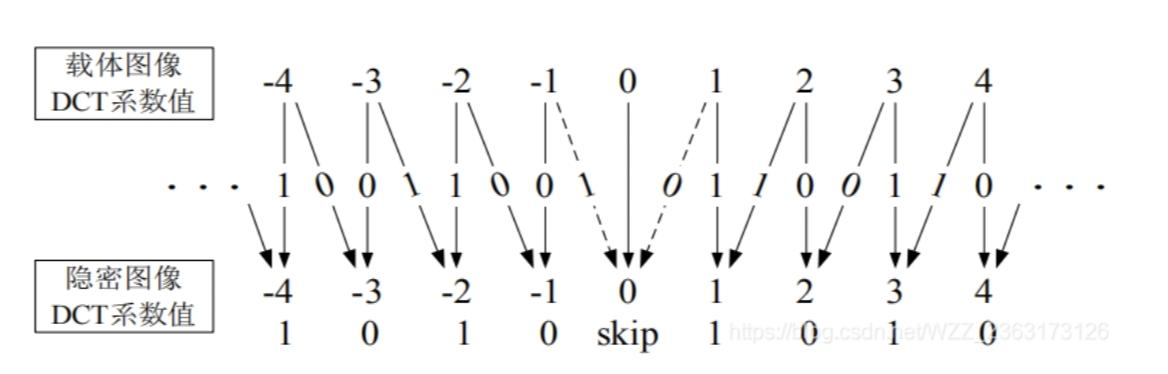
\includegraphics[width=\textwidth]{F4.jpg}
          \bottomcaption{\xiaowuhao{F4隐写规则}}
        \end{figure}\\
      \subsubsection{隐写后的分块逆DCT变换还原}
        在隐写结束后对每一个分块调用idct2函数进行DCT还原,再将原图和隐写后的图片进行输出,比较两者之间的差别。
      \subsubsection{F4隐写信息的提取}
        对于F4隐写信息后的图像,首先对其进行DCT变换,再比较每一个非零块,若为正奇数和负偶数则提取出1,
        若为正偶数和负奇数则提取出0,完成对隐写信息的提取。

    \subsection{实验2.2:F5隐写算法}
      \subsubsection{获取嵌入域}
        对输入图片的格式进行修改,在本次实验中使用的是png格式的图片,该种类型的图片大小为m*n*3,只取出其红色
        部分的像素块当作信息隐写的载体,在信息隐写结束再将隐写后的红色部分与其他两个色域进行混合最后输出结果。
      \subsubsection{位置置乱}
        首先指定位置置乱的密钥即为c\_a,c\_b,times的值,其中a和b为在置乱算法中要用到的参数,times为进行置乱的次数
        置乱时需要经过times次置乱循环,在每一次的循环中,遍历置乱前矩阵的各点的坐标x,y的值,通过运算算法\par
        $xx=mod((x-1)+c_b*(y-1),N)+1$ \par 
        $yx=mod(c_a*(x-1)+(c_a*c_b+1)*(y-1),N)+1$\par
        计算出该点的新坐标后将该点转移到新坐标的位置,在遍历完成后再继续进行下一轮的循环
      \subsubsection{编码参数确定}
        在本次实验中,选取每次嵌入信息的长度为3,因为选取的汉明码一致校验阵的大小为3*7,
        所以选择每次嵌入信息的载体长度为7,由此可以得到较高的嵌入效率
        
      \subsubsection{嵌入信息}
        开始嵌入信息后首先寻找JPEG图像中AC系数的非零值,在找到一个后将其坐标保存到变量sit中,sit变量
        保存着当前7个隐写载体的位置坐标。\par
        然后判断AC系数的值,若AC系数为正奇数或负偶数则在a矩阵的对应位置保存一个1;若AC系数为负奇数或正偶数
        则在a矩阵的对应位置保存一个0,a矩阵中保存着7个隐写载体所代表的值。\par
        在有7个隐写载体可隐写位时开始对载体进行隐写操作,首先计算要进行修改的位数,将汉明码一致校验阵M与载体
        矩阵a进行矩阵乘法运算,将得到的结果记为temp矩阵,然后取秘密信息的3位,记录在矩阵data\_bit中。
        然后将temp矩阵模2后与data\_bit进行按位异或操作,将得到的结果记为n,将n转为十进制表示即为要改写的位。\par
        如果得到要改写的位为0,则不用对隐写载体进行修改,若要改写的位n不为0,则要对载体矩阵a的第n位按照F4的
        隐写规则进行改写。\par
        在改写结束后需要判断改写后当前位置的AC系数是否为0,如果改写后的结果为0,则需要跳过该位,并且重新对取出的秘密信息进行隐写
        如果改写后的结果不为0则隐写完成,继续寻找能够隐写的载体隐写下一组秘密信息。

      \subsubsection{位置逆置乱}
        在隐写操作进行完毕后需要将位置置乱的结果进行逆操作,将DCT系数恢复到原来的顺序,在位置逆置乱的过程中同样采用
        循环的形式,经过times次循环对图像的JPEG系数进行逆置换,变换的运算算法如下所示\par
        $xx=mod((c_a*c_b+1)*(x-1)-c_b*(y-1),N)+1$\par
        $yy=mod(-c_a*(x-1)+(y-1),N)+1$\par
        在经过图像的逆置换后图像的JPEG系数的位置恢复到进行完DCT变换后的位置。
      \subsubsection{熵编码}
        按照JPEG标准对DCT系数调用函数idct进行逆DCT变换,然后由于原图为png图片,在逆dct变换后需要将得到的矩阵与原图的绿色蓝色部分的矩阵
        进行混合,然后得到的图像即为隐写之后的图像,完成对秘密信息的隐写操作。



\section{实验结果与分析:}

  \subsection{实验1.1:LSBM隐写算法}
    \begin{itemize}
      \item LSBM隐写结果
        运行LSBM隐写程序后会生成四个图像,其中第一列为原图和隐写后图像的对比,第二列为原图和隐写后图像的灰度直方图的对比便于分析值对效应
        \begin{figure}[H]
          \centering
          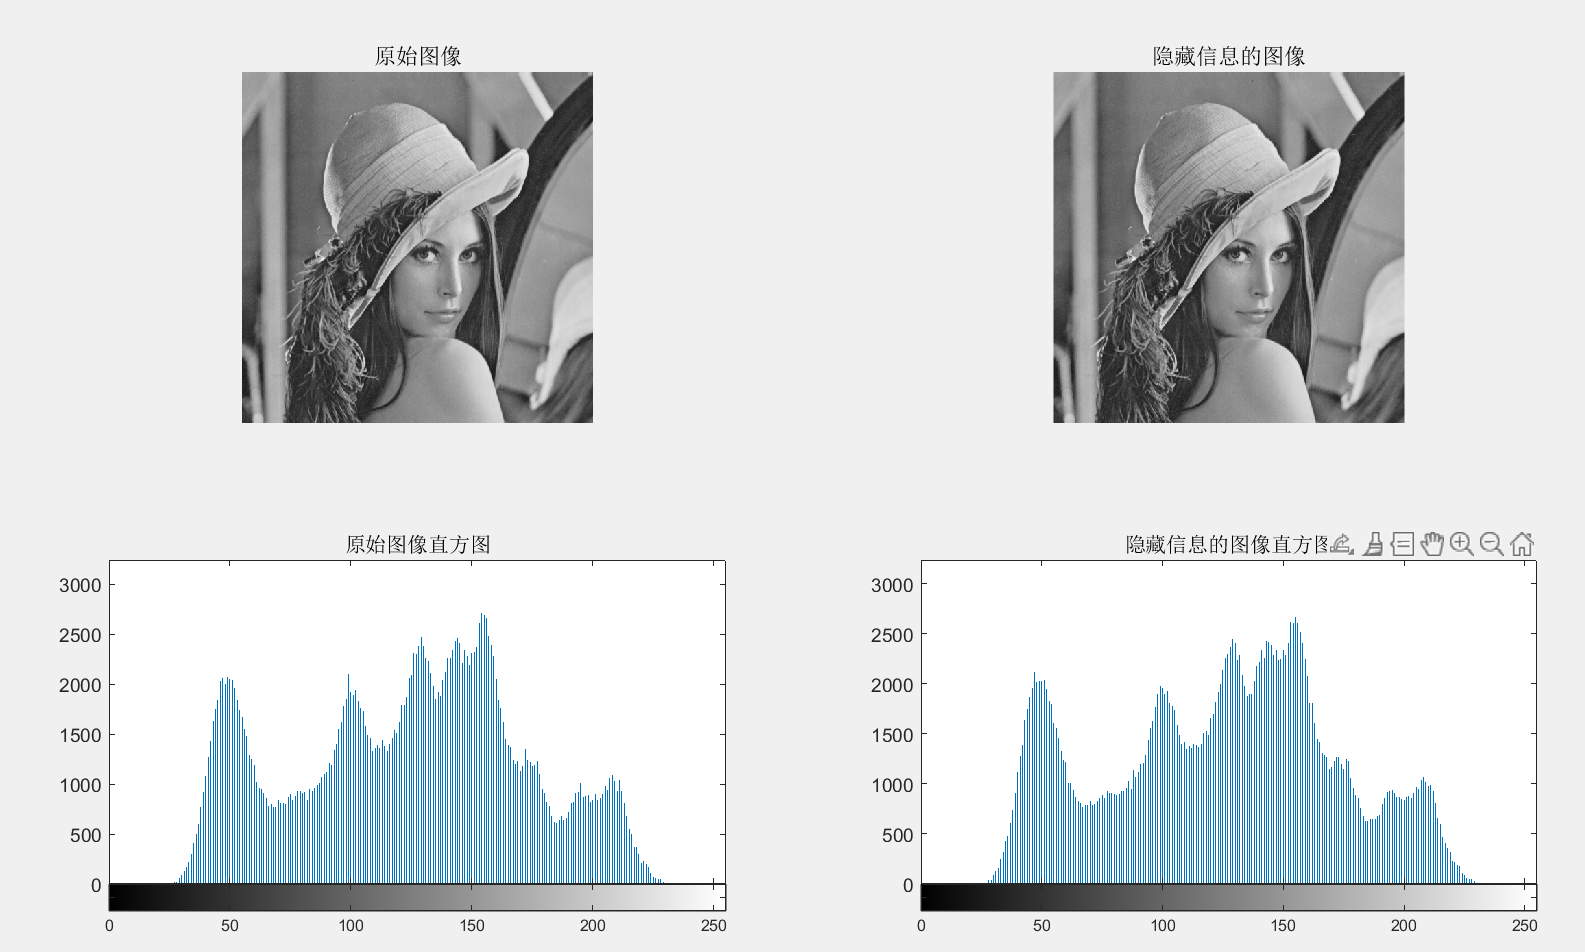
\includegraphics[width=\textwidth]{LSBM_hide.png}
          \bottomcaption{\xiaowuhao{LSBM隐写前后图像}}
        \end{figure}
        经过观察发现当隐写率为80\%时通过肉眼并不能看出明显的区别,观察两张图片的灰度直方图观察其值对效应发现隐写后的图像的较为不明显
\newpage
      \item LSBM隐写提取结果
        运行LSBM隐写提取秘密信息的程序后,得到的提取结果如下所示
        \begin{figure}[H]
          \centering
          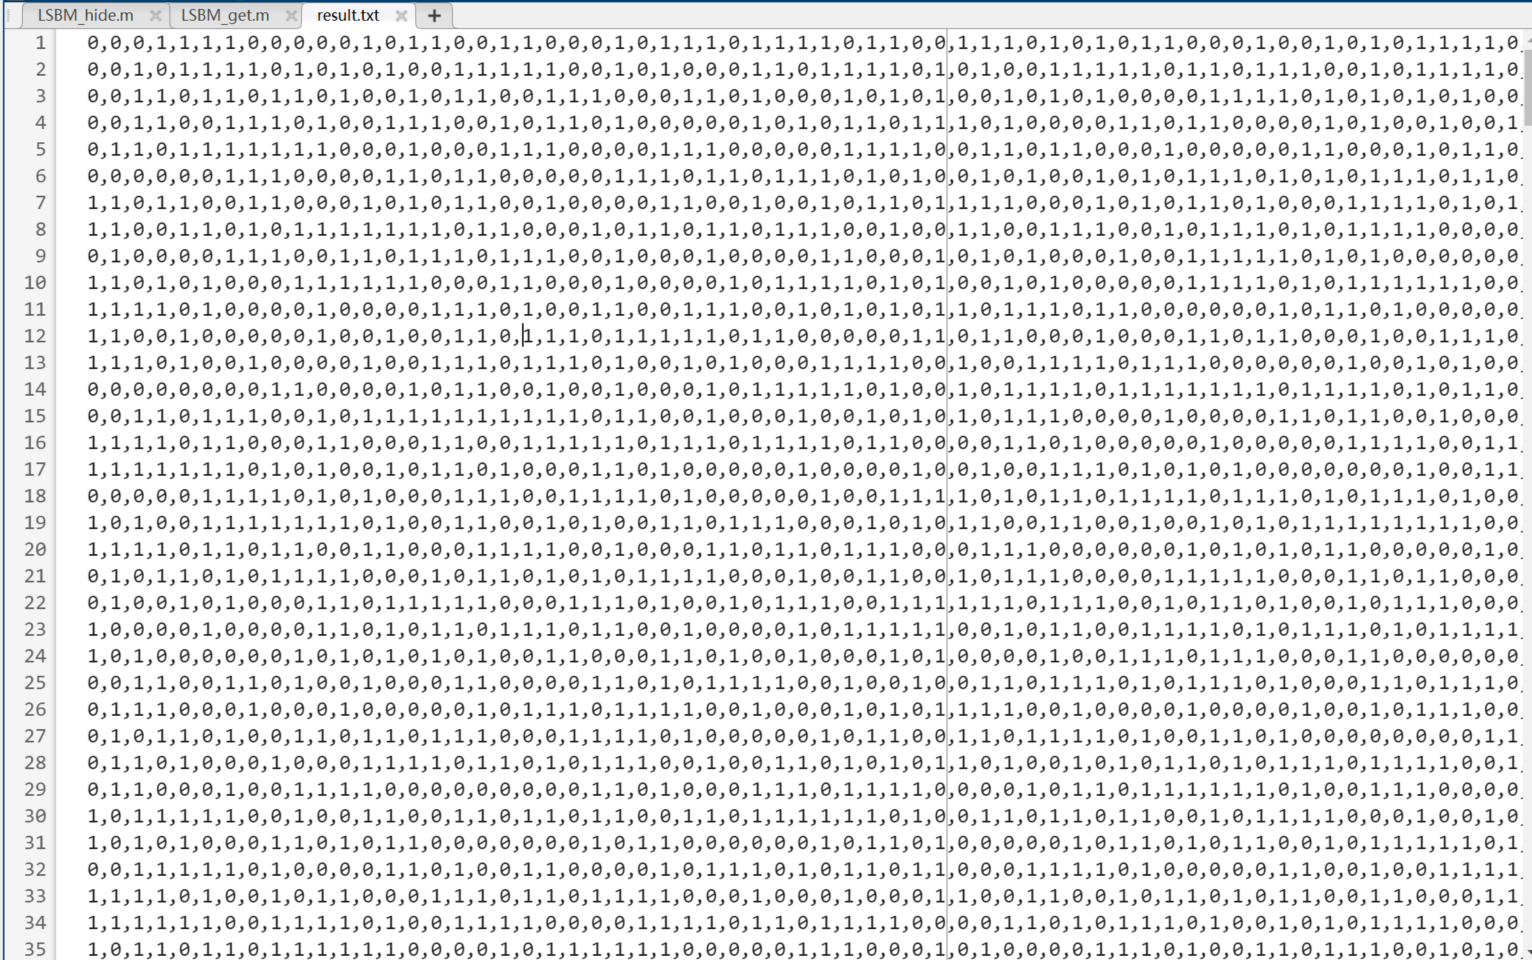
\includegraphics[width=13cm]{LSBM_get.png}
          \bottomcaption{\xiaowuhao{LSBM隐写提取结果}}
        \end{figure}

      \item 对LSBM隐写结果进行安全性分析
        对LSBM隐写结果进行卡方分析,当嵌入率为80\%时得到的卡方分析结果如下图所示\par
        \begin{figure}[H]
          \centering
          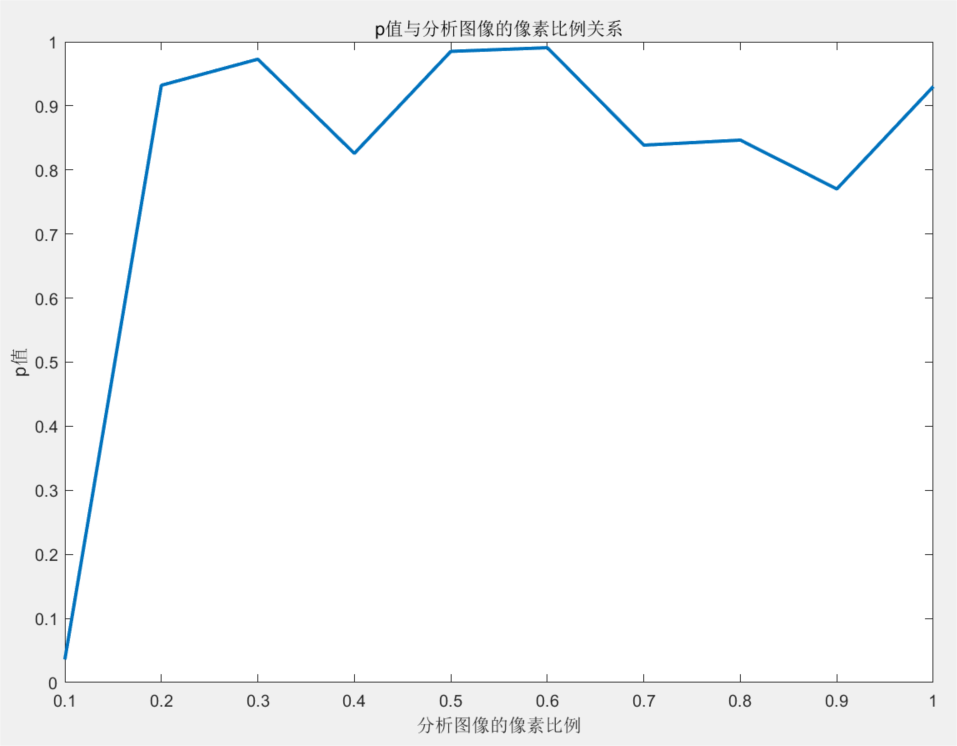
\includegraphics[width=11cm]{k2_LSBM_80.png}
          \bottomcaption{\xiaowuhao{对嵌入率为80\%的LSBM隐写图像卡方分析结果}}
        \end{figure}
        通过卡方分析结果我们可以得出当LSBM的嵌入率比较大达到80\%时,卡方分析仍然不能分析出是否有信息的隐写。可以认为LSBM隐写方法在
        对抗卡方分析时是安全的
    \end{itemize}

  \subsection{实验1.2:卡方分析}

    \subsubsection{对LSBR进行卡方分析}
      \begin{itemize}
        \item 对嵌入率为90\%的LSBR隐写结果进行卡方分析
        当LSBR的嵌入率是90\%时,得到的卡方分析结果如下图所示
        \begin{figure}[H]
          \centering
          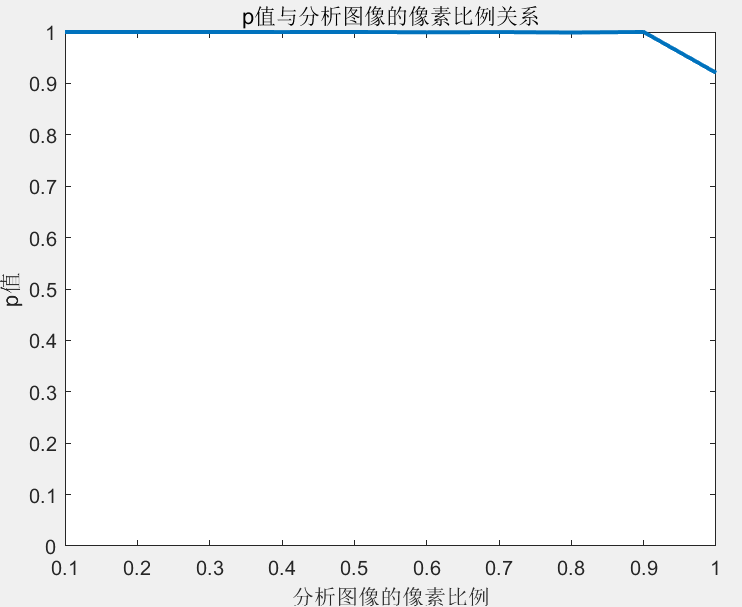
\includegraphics[width=11cm]{k2_LSBR_90.png}
          \bottomcaption{\xiaowuhao{对嵌入率为90\%的LSBR隐写图像卡方分析结果}}
        \end{figure}
        通过观察卡方分析的结果我们可以看出,p值曲线在图像像素比例0-0.9的区间内保持为1,而在0.9-1的区间内出现下降
        由此可以断定出该LSBR隐写的嵌入率为90\%。
\newpage
        \item 对嵌入率为50\%的LSBR隐写结果进行卡方分析
          当LSBR的嵌入率是50\%时,得到的卡方分析结果如下图所示
          \begin{figure}[H]
            \centering
            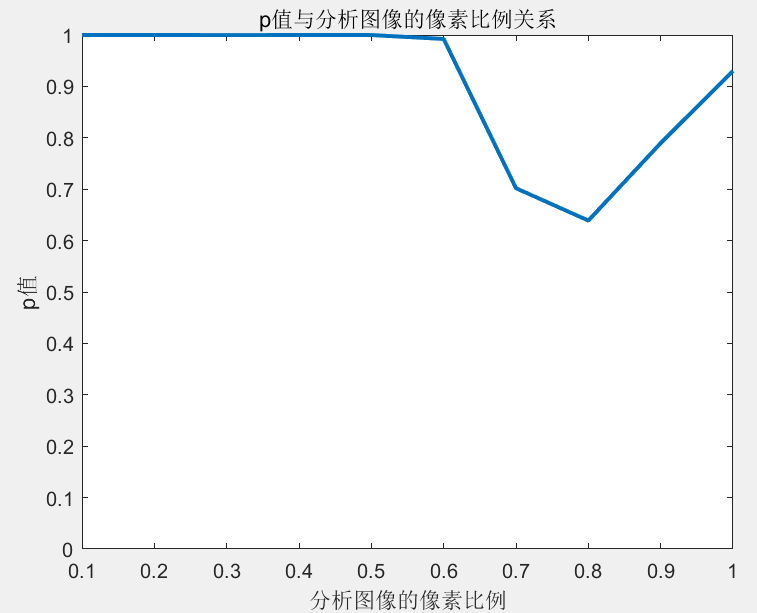
\includegraphics[width=9cm]{k2_LSBR_50.png}
            \bottomcaption{\xiaowuhao{对嵌入率为50\%的LSBR隐写图像卡方分析结果}}
          \end{figure}
          通过观察卡方分析的结果我们可以看出,p值曲线在图像像素比例0-0.5的区间内保持为1,而在0.6-1的区间内出现下降
          由此可以断定出该LSBR隐写的嵌入率为50\%。

        \item 对嵌入率为20\%的LSBR隐写结果进行卡方分析
          当LSBR的嵌入率为20\%时,得到的卡方分析结果如下图所示
          \begin{figure}[H]
            \centering
            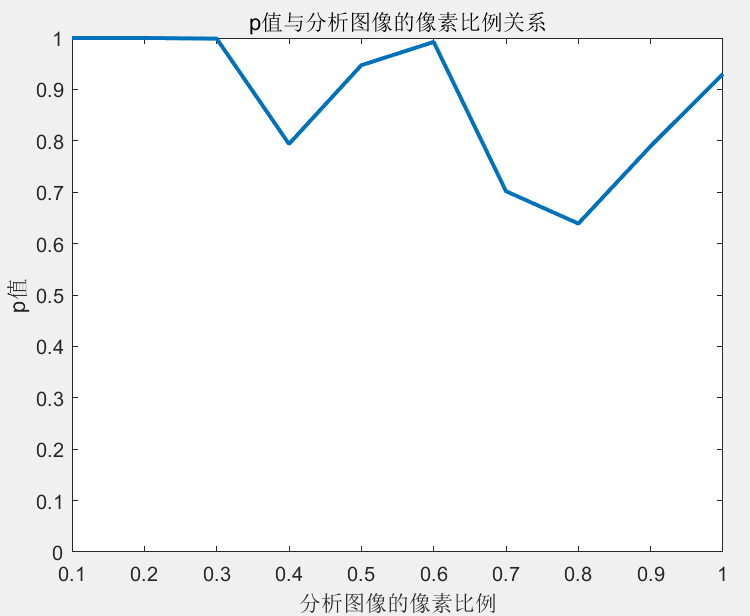
\includegraphics[width=9cm]{k2_LSBR_20.png}
            \bottomcaption{\xiaowuhao{对嵌入率为20\%的LSBR隐写图像卡方分析结果}}
          \end{figure}
          通过观察程序运行的结果我们可以看出,p值曲线在像素比例0-0.2的区间内保持为1,而在0.3-1的区间内出现下降
          由此可以断定出该LSBR隐写的嵌入率为20\%。

        \item 卡方分析对LSBR隐写的分析结果
          对LSBR嵌入率为20\%,50\%,90\%分别进行卡方分析可以得出结果,卡方分析可以分析出伪随机LSBR嵌入是否隐藏信息以及隐藏信息的长度
      \end{itemize}
    \subsubsection{对LSBM进行卡方分析}
      \begin{itemize}
        \item 对嵌入率是90\%的LSBM隐写结果进行卡方分析
          当LSBM的嵌入率是90\%时,得到的卡方分析结果如下图所示
          \begin{figure}[H]
            \centering
            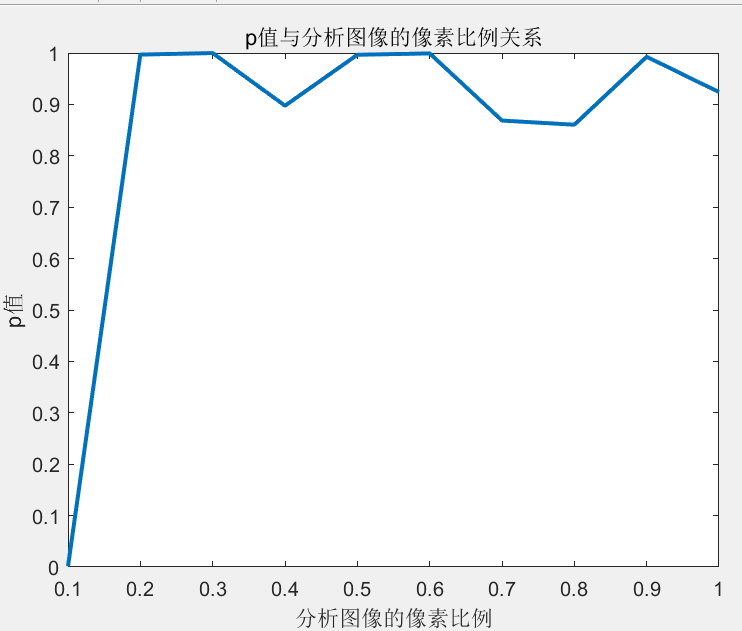
\includegraphics[width=11cm]{k2_LSBM_90.png}
            \bottomcaption{\xiaowuhao{对嵌入率为90\%的LSBM隐写图像卡方分析结果}}
          \end{figure}
          通过观察程序运行结果图像我们并不能看出p值曲线在像素比例下的变化趋势,并不能判断出图像是否嵌入信息以及信息的嵌入率是多少
\newpage
        \item 对嵌入率是50\%的LSBM隐写结果进行卡方分析
        当LSBM的嵌入率是50\%时,得到的卡方分析结果如下图所示
        \begin{figure}[H]
          \centering
          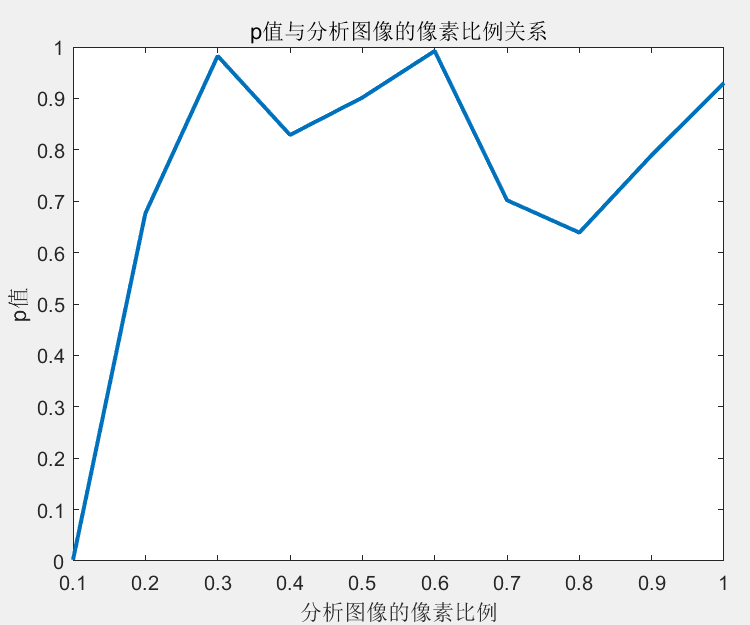
\includegraphics[width=9cm]{k2_LSBM_50.png}
          \bottomcaption{\xiaowuhao{对嵌入率为50\%的LSBM隐写图像卡方分析结果}}
        \end{figure}
        通过观察程序运行结果图像我们并不能看出p值曲线在像素比例下的变化趋势,并不能判断出图像是否嵌入信息以及信息的嵌入率是多少

        \item 对嵌入率是20\%的LSBM隐写结果进行卡方分析
        当LSBM的嵌入率是20\%时,得到的卡方分析结果如下图所示
        \begin{figure}[H]
          \centering
          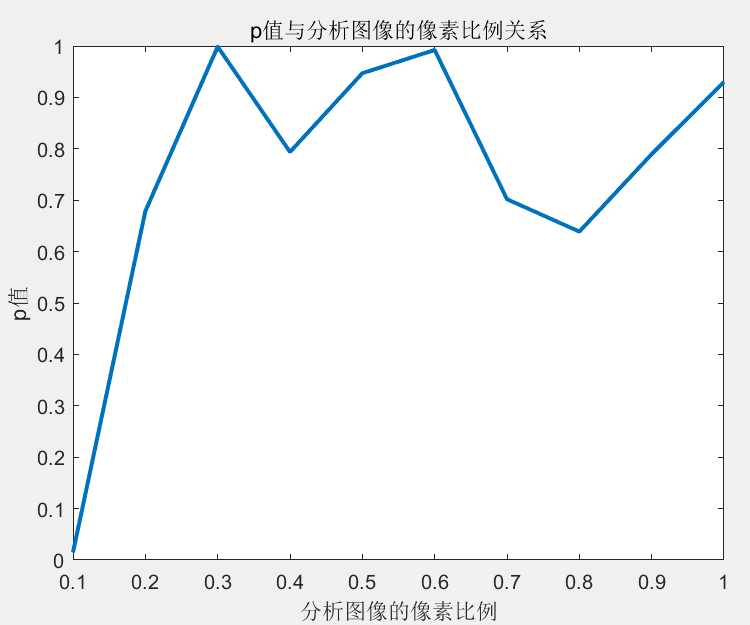
\includegraphics[width=9cm]{k2_LSBM_20.png}
          \bottomcaption{\xiaowuhao{对嵌入率为20\%的LSBM隐写图像卡方分析结果}}
        \end{figure}
        通过观察程序运行结果图像我们并不能看出p值曲线在像素比例下的变化趋势,并不能判断出图像是否嵌入信息以及信息的嵌入率是多少

        \item 卡方分析对LSBR隐写的分析结果
        对LSBM嵌入率为20\%,50\%,90\%分别进行卡方分析可以得出结果,卡方分析不能分析出LSBM嵌入是否隐藏信息以及隐藏信息的长度
      \end{itemize}

  \subsection{实验2.1:F4隐写算法}

    \begin{itemize}

      \item 对lena的png图像进行F4隐写得到的原图与隐写后的图像如下图所示
        \begin{figure}[H]
          \centering
          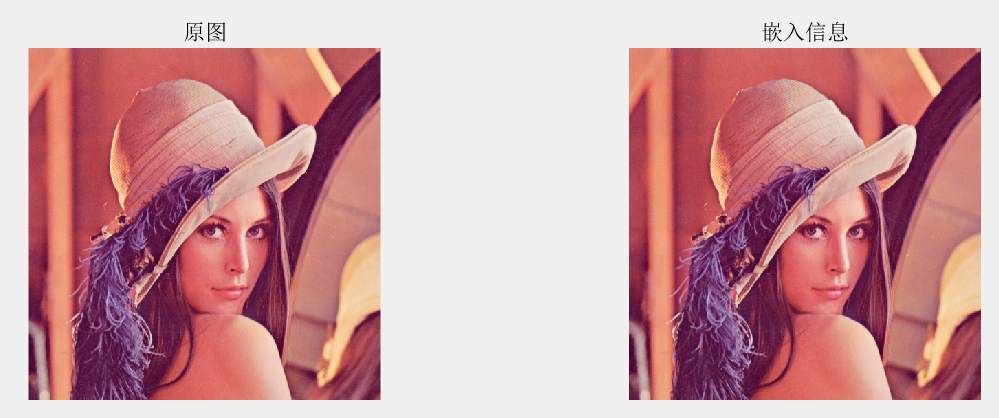
\includegraphics[width=10cm]{F4_image_compare.png}
          \bottomcaption{\xiaowuhao{F4隐写过后原图与隐写后图像的对比}}
        \end{figure}
        通过观察图像可以得出F4隐写后的图像仅凭人眼无法识别。

      \item  对lena图像进行F4隐写前后得到的图像的直方图对比如下图所示
        \begin{figure}[H]
          \centering
          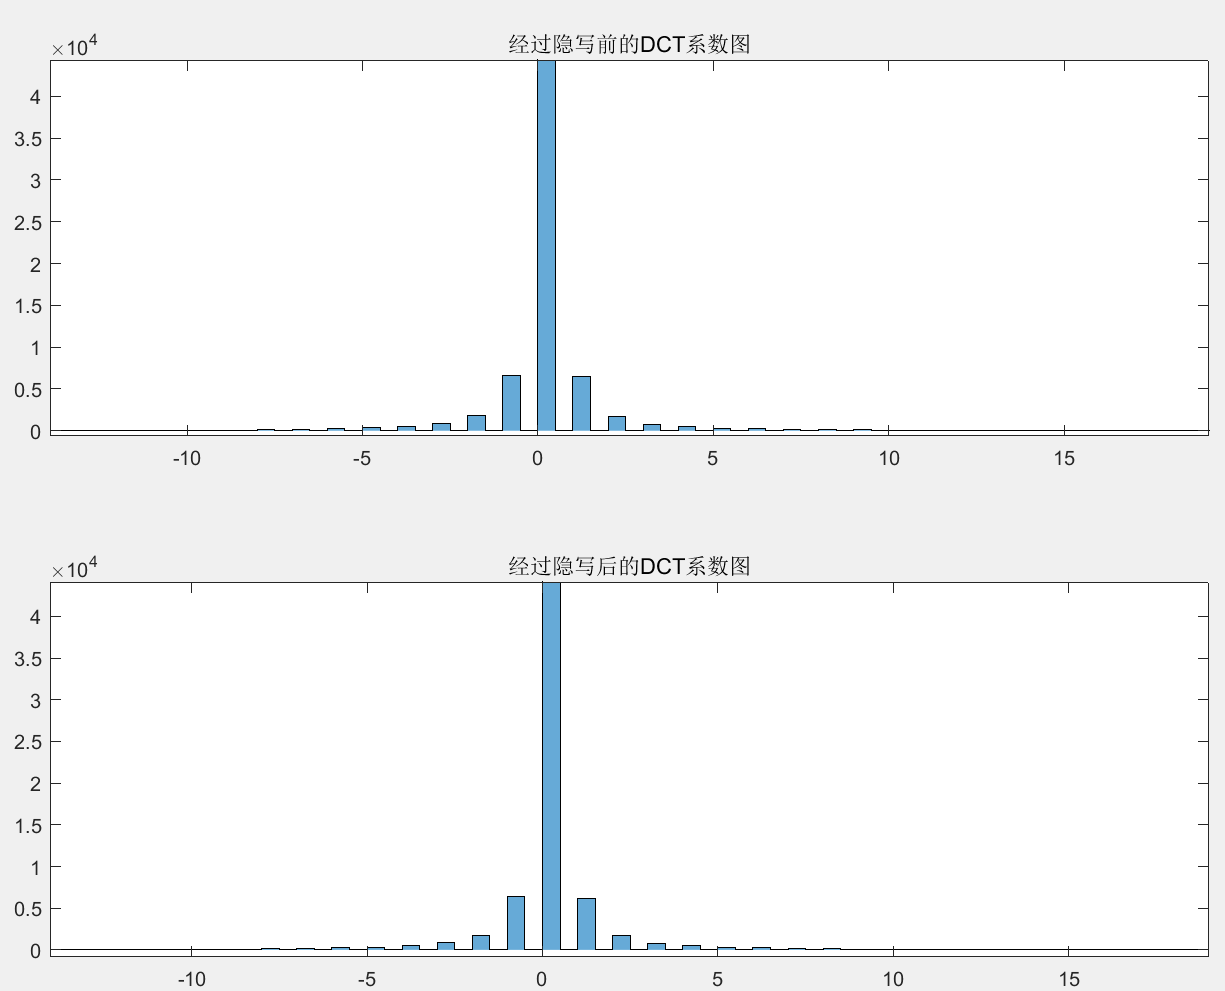
\includegraphics[width=10cm]{F4_hist_compare.png}
          \bottomcaption{\xiaowuhao{F4隐写过后原图与隐写后图像直方图的对比}}
        \end{figure}
        通过观察F4隐写后的直方图可以发现,经过F4隐写过后的图片并不存在值对效应,而且相比于F3的替换算法
        并不会使载密图像DCT系数中的偶系数增多。
        
      \item 对F4隐写后的图像进行信息提取得到的结果如下图所示
        \begin{figure}[H]
          \centering
          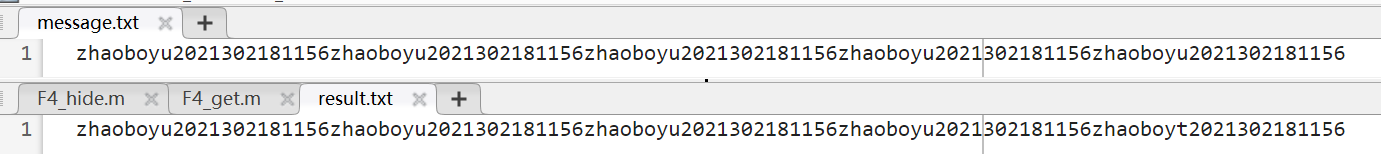
\includegraphics[width=11cm]{F4_get.png}
          \bottomcaption{\xiaowuhao{提取F4隐写后的图像的结果}}
        \end{figure}
        通过观察提取结果可以发现,该隐写方法并不能够将信息完整的提取出来,而是存在有一定的误码率。

      \item 将F4隐写后的图像进行安全性分析
        将F4隐写过后的图像输入到卡方分析程序中得到的分析结果如下图所示
        \begin{figure}[H]
          \centering
          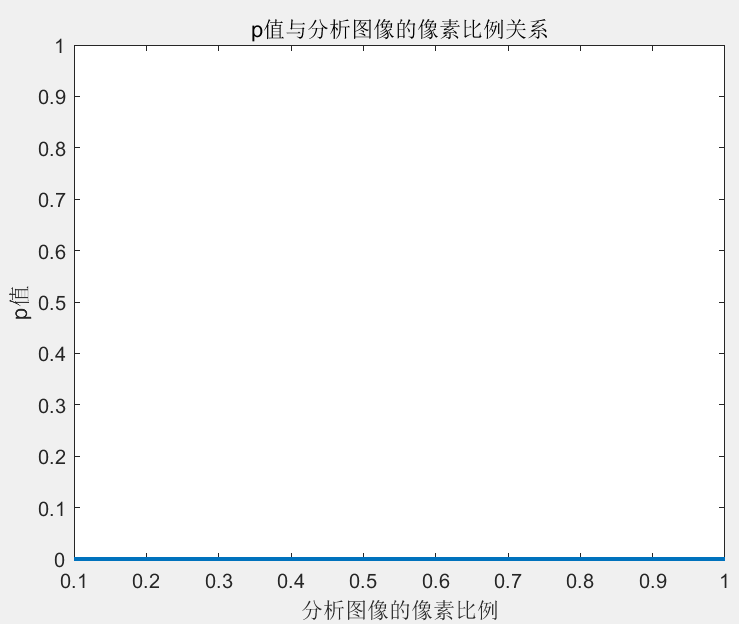
\includegraphics[width=11cm]{k2_F4.png}
          \bottomcaption{\xiaowuhao{对F4隐写后的结果进行卡方分析}}
        \end{figure}
        观察卡方分析结果,p值恒为0没有变化,可以得出结论F4隐写能够对抗卡方分析的检测,在卡方分析下具有安全性。
        
    \end{itemize}
\newpage
  \subsection{实验2.2:F5隐写算法}

    \begin{itemize}
      \item 将图像进行F5隐写过后生成的载密图像与原图像的对比如下图所示
        \begin{figure}[H]
          \centering
          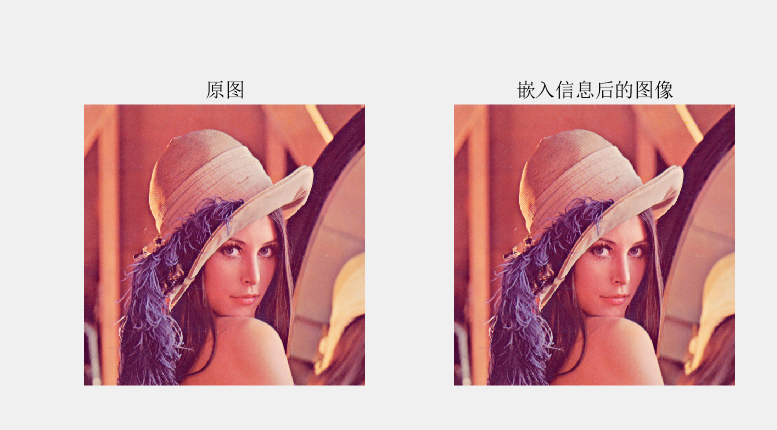
\includegraphics[width=9cm]{F5_image_compare.png}
          \bottomcaption{\xiaowuhao{对F5隐写后的原图与载密图像的对比}}
        \end{figure}

      \item 对F5隐写后的图像进行信息提取得到的结果如下图所示
        \begin{figure}[H]
          \centering
          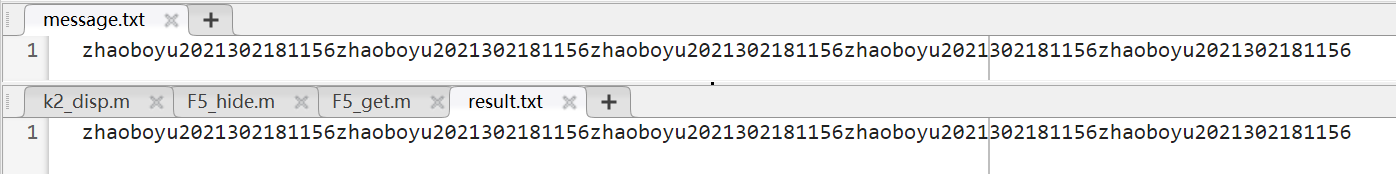
\includegraphics[width=11cm]{F5_get.png}
          \bottomcaption{\xiaowuhao{提取F5隐写后的图像的结果}}
        \end{figure}
        观察提取结果可得该隐写方法能够将隐写信息完整的提取出来

      \item 对F5隐写算法进行安全性分析
        对F5隐写算法后的载密图像进行卡方分析得到的结果如下图所示
        \begin{figure}[H]
          \centering
          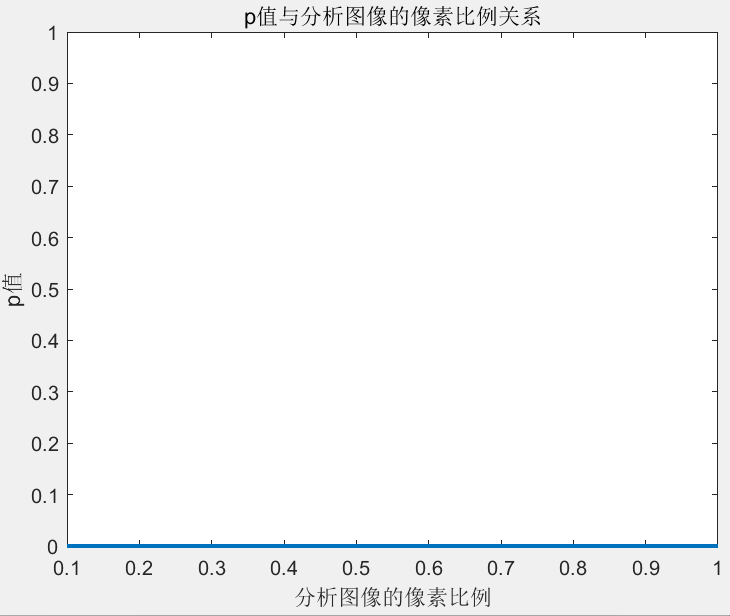
\includegraphics[width=9cm]{k2_F5.png}
          \bottomcaption{\xiaowuhao{F5隐写后的载密图像进行卡方分析}}
        \end{figure}
        观察卡方分析结果,p值恒为0没有变化,可以得出结论F5隐写能够对抗卡方分析的检测,在卡方分析下具有安全性。


      \item 对F5隐写结果修改的次数进行比较分析
        对LSBR,LSBM,F4,F5隐写算法中修改的数量进行统计,统计结果如下表所示

        \begin{table}[H]
          \caption{每种隐写方案修改次数统计}\label{tab1}
            \centering
          \begin{tabular*}{0.75\textwidth}{@{\extracolsep{\fill}}lccc}
              \toprule
              隐写方法          &隐写信息长度(bit)        &修改次数         &每次修改隐写信息长度                \\
              \midrule
              LSBR             &235929                    &236032          &0.9996                             \\
              LSBM             &52428                     &26109           &2.0080                             \\
              F4               &840                       &1324            &0.6344                              \\
              F5               &840                       &472             &1.7797                           \\ 
              \bottomrule
          \end{tabular*}
        \end{table}
        上述统计结果中LSBR的嵌入率为90\%,LSBM的嵌入率为20\%。\par
        通过比较结果我们可以得出在四种隐写方法中LSBM每次修改能够隐写的信息的长度最多,而F4每次修改能够隐写的信息长度最少
        F5每次修改隐写信息长度相比较于F4有非常大的提高,而且其安全性也明显高于LSBR和LSBM隐写算法。\par
        因此F5隐写算法能够保持在相对安全的前提下能够每次修改更多隐写信息

    \end{itemize}

\section{总结及心得体会:}
  1.在本次实验中学习到了LSBM隐写算法的操作方法以及其相对于LSBR隐写算法的改进效果。\par
  2.在本次实验中学习到了卡方分析这一检测信息隐写的方法,学会了使用其分析LSBR得到隐写的嵌入率的方法\par
  3.学习到了F4隐写算法的实现方法,了解到F4隐写算法相对于Jsteg隐写算法不仅消除了值对效应,相对于F3算法消除了隐写后偶系数变多的效应.\par
  4.学习到了F5隐写算法的实现方法,了解到通过汉明码一致校验阵进行信息的隐藏来减少每个载体分组中修改次数从而提高嵌入率的方法。\par
  5.体会到信息的安全隐写隐藏和隐写信息的检测与分析是相辅相成共同进步的关系,二者在对抗中不断进行功能的完善和效率的提高\par
  6.体会到了任何的隐写算法都会造成载密图像与原图像之间的差别,并不存在一种完全不能被检测出来的隐写算法,但只存在有更为安全的能够
  对抗更多分析算法的隐写算法。\par


\vspace{4cm}

\end{document}





    

  



